\documentclass[10pt,final,a4paper,oneside,onecolumn]{article}

%%==========================================================================
%% Packages
%%==========================================================================
\usepackage[a4paper,left=3.5cm,right=3.5cm,top=3cm,bottom=3cm]{geometry} %% change page layout; remove for IEEE paper format
\usepackage[T1]{fontenc}                        %% output font encoding for international characters (e.g., accented)
\usepackage[cmex10]{amsmath}                    %% math typesetting; consider using the [cmex10] option
\usepackage{amssymb}                            %% special (symbol) fonts for math typesetting
\usepackage{amsthm}                             %% theorem styles
\usepackage{dsfont}                             %% double stroke roman fonts: the real numbers R: $\mathds{R}$
\usepackage{mathrsfs}                           %% formal script fonts: the Laplace transform L: $\mathscr{L}$
\usepackage[pdftex]{graphicx}                   %% graphics control; use dvips for TeXify; use pdftex for PDFTeXify
\usepackage{array}                              %% array functionality (array, tabular)
\usepackage{upgreek}                            %% upright Greek letters; add the prefix 'up', e.g. \upphi
\usepackage{stfloats}                           %% improved handling of floats
\usepackage{multirow}                           %% cells spanning multiple rows in tables
%\usepackage{subfigure}                         %% subfigures and corresponding captions (for use with IEEEconf.cls)
\usepackage{subfig}                             %% subfigures (IEEEtran.cls: set caption=false)
\usepackage{fancyhdr}                           %% page headers and footers
\usepackage[official,left]{eurosym}             %% the euro symbol; command: \euro
\usepackage{appendix}                           %% appendix layout
\usepackage{xspace}                             %% add space after macro depending on context
\usepackage{verbatim}                           %% provides the comment environment
\usepackage[dutch,USenglish]{babel}             %% language support
\usepackage{wrapfig}                            %% wrapping text around figures
\usepackage{longtable}                          %% tables spanning multiple pages
\usepackage{pgfplots}                           %% support for TikZ figures (Matlab/Python)
\pgfplotsset{compat=1.14}						%% Run in backwards compatibility mode
\usepackage[breaklinks=true,hidelinks,          %% implement hyperlinks (dvips yields minor problems with breaklinks;
bookmarksnumbered=true]{hyperref}   %% IEEEtran: set bookmarks=false)
%\usepackage[hyphenbreaks]{breakurl}            %% allow line breaks in URLs (don't use with PDFTeX)
\usepackage[final]{pdfpages}                    %% Include other pdfs
\usepackage[capitalize]{cleveref}				%% Referensing to figures, equations, etc.
\usepackage{units}								%% Appropriate behavior of units
\usepackage[utf8]{inputenc}   				 	%% utf8 support (required for biblatex)
\usepackage{csquotes}							%% Quoted texts are typeset according to rules of main language
\usepackage[style=ieee,doi=false,isbn=false,url=false,date=year,minbibnames=15,maxbibnames=15,backend=biber]{biblatex}
%\renewcommand*{\bibfont}{\footnotesize}		%% Use this for papers
\setlength{\biblabelsep}{\labelsep}
\bibliography{../../bib}

%%==========================================================================
%% Define reference stuff
%%==========================================================================
\crefname{figure}{Figure}{Figures}
\crefname{equation}{}{}

%%==========================================================================
%% Define header/title stuff
%%==========================================================================
\newcommand{\progressreportnumber}{23}
\renewcommand{\author}{Erwin de Gelder}
\renewcommand{\date}{16 October 2019}
\renewcommand{\title}{Performance assessment of automated vehicles using real-world driving scenarios}

%%==========================================================================
%% Fancy headers and footers
%%==========================================================================
\pagestyle{fancy}                                       %% set page style
\fancyhf{}                                              %% clear all header & footer fields
\fancyhead[L]{Progress report \progressreportnumber}    %% define headers (LE: left field/even pages, etc.)
\fancyhead[R]{\author, \date}                           %% similar
\fancyfoot[C]{\thepage}                                 %% define footer

\begin{document}
	
\begin{center}
	\begin{tabular}{c}
		\title \\ \\
		\textbf{\huge Progress report \progressreportnumber} \\ \\
		\author \\ 
		\date
	\end{tabular}
\end{center}



\section{Previous meeting minutes}

\begin{itemize}
	\item We discussed the plan for the \emph{scenario risk estimation}. Olaf had a suggestion for similar type of studies focusing on passive safety. Jan-Pieter suggested that other people at TNO did already significant work for the extraction of scenarios, so I could use that work for the case study.
\end{itemize}



\section{Summary of work}

\begin{itemize}
	\item I received feedback on our manuscript of the \emph{ontology article}. We are asked to provide a major revision. I wrote a cover letter in which I explain how we (are going to) address the comments of the reviewers.
	
	\item Because this meeting is a \emph{yearly progress meeting}, I summarized the work done together with an outlook for next year in \cref{sec:work}. In \cref{sec:evaluation}, reflect on my progress last year.
	
	\item I am back to the Netherlands. I will continue working on Singaporean projects. Therefore, in the coming six months, I will still travel to Singapore. However, the majority of the time, I will be in the Netherlands. 
\end{itemize}



\section{Work and outlook}
\label{sec:work}

I worked on several topics last year. Here follows a list of the topics I worked on:
\begin{itemize}
	\item Quantifying the completeness of a dataset that is used to extract scenarios for the assessment of automated vehicles. The work is published in a special issue of the Traffic Injury Prevention journal \cite{degelder2019completeness}.
	
	I guided a student on this topic. The student applied methods for the estimation of the number of species \cite{chao1992estimating, chao1993stopping} for estimating the number of ``scenario classes''. I do not think the student's work is mature enough for a paper.
	
	\item Estimating the risk of a scenario for a specific automated driving system. With the help of two colleagues, I wrote a conference paper in which we proposed a method to estimate the risk of a scenario (category) associated with an automated driving system \cite{degelder2019risk}.
	
	\item Ontology for scenarios for the assessment of automated vehicles. I wrote a journal paper that is submitted to Transportation Research Part C: Emerging Technologies.
	
	\item In CETRAN, Singapore, Olaf and I worked on a strategy for assessing autonomous vehicles.
\end{itemize}

The updated planning is shown in \cref{fig:planning}. For next year, I plan to work on the following:
\begin{itemize}
	\item I want to get our ontology paper published soon.
	
	\item I want to publish about the work on the strategy for assessing autonomous vehicles. I aim for a conference paper for the FISITA world congress\footnote{Abstract deadline November 30, 2019, paper deadline May 1, 2020.}. To make a journal paper out of it, I think we need to apply the strategy on a real car. I have my doubts whether this is feasible or not and, thus, I doubt if we can make it to a journal paper.
	
	\item I want to continue our work on the risk estimation for scenarios. Part of this study is the extraction of different scenarios in a dataset and the likelihood estimation of the scenarios. Part of this work has been done by colleagues based on (growing) n-grams \cite{kneser1995improved}. Documentation is lacking and it would be too much to also describe these methods in detail in one article with the risk estimation. Therefore, I want to write two conference papers about this subject together with my colleagues:
	\begin{itemize}
		\item Using n-grams for mining of traffic scenarios.
		\item Estimating the likelihood of seen and unseen traffic scenarios.
	\end{itemize}
	Initially, we can aim for the Intelligent Vehicle Symposium (IV)\footnote{Paper deadline January 30, 2020.}. The Intelligent Transportation Systems Conference (ITSC) could be a backup\footnote{Paper deadline February 28, 2020.}.
	
	After these conference papers, I will continue the work on the risk estimation.
	
	\item I will have a student starting in January 2020. The student will work on the generation of test cases. I do not plan to work on that topic myself for the coming period.
\end{itemize}

\begin{figure}
	\centering
	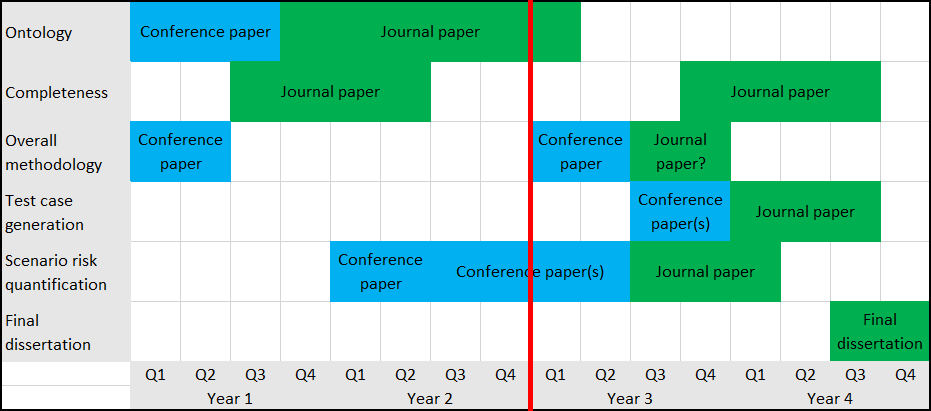
\includegraphics[width=\linewidth]{planning.png}
	\caption{Proposed planning at the second yearly progress meeting. The red line indicated the time of writing this report.}
	\label{fig:planning}
\end{figure}



\section{Self-reflection of second year}
\label{sec:evaluation}

Most importantly, I am still enjoying my PhD. I am eager to continue working on the different topics and to write papers about the work. There is, however, always some room for improvement. The following list addresses three topics that need attention:
\begin{itemize}
	\item \emph{Time, expectation, and stakeholder management}: One year ago, I mentioned time, expectation, and stakeholder management in my self-reflection. Although I see some improvement, this still needs attention. More specifically, I underestimate the time I need for a specific task. This, in turn, leads to too high expectation. Furthermore, because my planning is often too ambitious, I cannot satisfy all stakeholders. 
	
	I hope that with extra attention and some coaching, I will further improve my time, expectation, and stakeholder management.
	
	\item \emph{Overall progress}: I hoped to have more progress during last year in terms of the papers I have written. I spent significant time on work that is not (yet) publishable. 
	
	Next year, I will try to focus more on disseminating my work through (conference) papers. 
	
	\item \emph{Focus of work}: Initially, I planned to focus more on analyzing data for the extraction and generation of scenarios for the assessment of automated vehicles. Due to the lack of data in Singapore, I shifted the focus. As a result, I worked a lot on the strategy for assessing autonomous vehicles. Now that I am back in the Netherlands, I have the feeling that I am lacking behind in terms of the technology/tools we have developed for the data mining of scenarios. 
	
	Next year, I hope to catch up by focusing my attention also on the data mining and the generation of scenarios. 
\end{itemize}




\printbibliography

\clearpage
\includepdf[pages=-,pagecommand={},width=\paperwidth]{../../"20191004 Ontology revision letter"/ontology_revision.pdf}

\end{document}